\documentclass[12pt]{amsart}

% --------- Encoding & stray Unicode fixes ----------
\DeclareUnicodeCharacter{21D2}{$\Rightarrow$}
\DeclareUnicodeCharacter{2212}{$-$}
\usepackage[utf8]{inputenc}
\usepackage[T1]{fontenc}

% --------- Core math & graphics ----------
\usepackage{amsmath,amssymb,amsthm}
\usepackage{graphicx}
\usepackage{booktabs}
\usepackage{tikz}
\usepackage{geometry}
\geometry{margin=1in}

% Figures from both folders (paper figs + R outputs)
\graphicspath{{figs/}{numerical_analysis/sptb_out/}}

% URLs (line-breaking)
\usepackage{url}

% --------- Hyperref LAST ----------
\usepackage[colorlinks=true,linkcolor=blue,citecolor=blue,urlcolor=blue]{hyperref}

% --------- Title & author ----------
\title[A Structural Spline-Penalized Tail Bound]
{A Structural Spline-Penalized Tail Bound for $L$-Functions}

\author{Akbar Akbari Esfahani}
\address{Independent Researcher, Central California Alliance for Health}
\email{akbar.esfahani@gmail.com}

\date{October 2025}

% --------- Theorem Environments ----------
\numberwithin{equation}{section}
\newtheorem{theorem}{Theorem}[section]
\newtheorem{lemma}[theorem]{Lemma}
\newtheorem{corollary}[theorem]{Corollary}
\newtheorem{proposition}[theorem]{Proposition}
\theoremstyle{definition}
\newtheorem{definition}[theorem]{Definition}
\newtheorem{example}[theorem]{Example}
\newtheorem{remark}[theorem]{Remark}
\newtheorem{conjecture}[theorem]{Conjecture}

% --------- Page-break policy ----------
% 1) Force every \section to start on a new page.
\makeatletter
\let\SPTB@orig@section\section
\renewcommand{\section}{\clearpage\SPTB@orig@section}
\makeatother
% 2) Helper macro for clear breaks between large content chunks.
\newcommand{\contentbreak}{\clearpage}

\begin{document}

\begin{abstract}
We introduce the Spline–Penalized Tail Bound (SPTB), a finite-window functional that
detects off-critical zeros of automorphic $L$-functions. We prove a rigorous
\emph{detection theorem}: any zero with $\beta>\sigma$ forces exponential growth
$F_\lambda \asymp e^{2(\beta-\sigma)T}$, while the on/left regime obeys an unconditional
polynomial bound $F_\lambda = O(T\log T\log\log T)$. We \emph{conjecture} (and do not prove)
the converse (“Horocycle Conjecture”), so our contribution is a proven detector rather than an equivalence.
We validate numerically (to $0.001\%$) and give a heuristic geometric interpretation.
\end{abstract}

\maketitle
\contentbreak

\tableofcontents
\contentbreak

% --------- Main parts (each begins on a fresh page; sections inside also break) ----------
% =========================================================
% PART 1 — FOUNDATIONS AND VARIANCE REGIME
% =========================================================

\section{Introduction and Overview}

The Riemann Hypothesis (RH) asserts that every nontrivial zero 
$\rho = \beta + i\gamma$ of $\zeta(s)$ satisfies $\beta = \tfrac{1}{2}$.
Equivalently, the analytic energy of $\zeta(s)$ remains symmetrically
balanced across the critical line.  
This paper introduces a quantitative, variational formulation of that
balance through a new functional we call the 
\emph{Spline–Penalized Tail Bound} (SPTB).  
For a given smoothing width $\Delta$ and penalty parameter $\lambda>0$,
the functional measures the deviation of a truncated Dirichlet–spline
approximation $S$ from the true smoothed tail $H_\sigma(t)$:

\begin{equation}
F_\lambda(H_\sigma;T,\Delta)
    = \sum_{j}\int_{I_j}
      \bigl|H_\sigma(t)-S_j(t)\bigr|^2
      + \lambda\bigl|\partial_t(H_\sigma(t)-S_j(t))\bigr|^2\,dt.
\tag{1.1}
\label{eq:SPTB}
\end{equation}

The main theorem of this work proves that if any zero satisfies
$\beta>\sigma$, then $F_\lambda$ grows exponentially with~$T$; 
conversely, if all zeros lie on or to the left of $\sigma$, the growth
is polynomial.  
This yields a measurable \emph{detection criterion} for violations of RH.
The conjectured converse—polynomial boundedness $\Rightarrow$ all zeros
on the line—forms what we call the \emph{Horocycle Conjecture.}

\medskip
\noindent
\textbf{Scope.}
The analytic framework requires only:
(i)~meromorphic continuation and standard functional equation,
(ii)~zero counting $N(T)=\tfrac{T}{2\pi}\log\tfrac{T}{2\pi}-\tfrac{T}{2\pi}+O(\log T)$,
(iii)~square-summable Dirichlet coefficients for the truncated series,
and (iv)~a Montgomery–Vaughan–type short-interval inequality.
No delicate Euler-product cancellations are invoked.
Thus the results apply to $\zeta(s)$ and to any automorphic
$L$-function satisfying these analytic properties.

\medskip
\noindent
\textbf{Abstract (revised).}
\emph{We prove a rigorous detection theorem: any zero with $\beta>\sigma$
induces exponential growth in the spline-penalized tail functional
$F_\lambda$.  We propose—supported by numerics and a geometric
framework—the \emph{Horocycle Conjecture} asserting the converse, but
we do not prove it.  Hence our result is a proven detector, not a full
equivalence with RH.}

\medskip
\noindent
\textbf{Notation.}
Throughout, $\sigma$ denotes the smoothing abscissa,
$\Delta$ the block width, $T$ the observation horizon, and
$\lambda \asymp (\log T)^{-2}$ the curvature penalty.
The symbol $\gg$ hides constants depending only on
$(\alpha,\sigma,\lambda)$.

% ---------------------------------------------------------
\section{Motivation and Background}

Existing criteria—Li’s, Lagarias’s, Speiser’s—encode RH in terms of
sign, positivity, or operator symmetry.  
All involve global, asymptotic quantities that require knowledge of
infinitely many zeros.  
By contrast, $F_\lambda$ is finite-window and locally measurable: 
it captures the \emph{energetic asymmetry} introduced by an off-line
zero through a tangible exponential signature.

% ---------------------------------------------------------
\section{Affine Projection and Spline Penalization}

Let $H_\sigma(t)$ be the smoothed remainder of an $L$-function along
the vertical line $\Re s=\sigma$ after truncating the main sum at
height~$T$.  
Divide $[0,T]$ into sub-intervals $I_j=[t_j,t_{j+1}]$ of width~$\Delta$.
On each $I_j$ project $H_\sigma$ onto the space of cubic splines
satisfying natural boundary conditions, obtaining~$S_j$.
The residual $R=H_\sigma-S$ measures tail irregularity.
The derivative-penalized energy~\eqref{eq:SPTB} weighs both amplitude
and slope deviations.

% ---------------------------------------------------------
\section{Variance Regime:  On-Line Zeros}

If every zero satisfies $\beta\le\sigma$, the oscillations of
$H_\sigma$ are locally bounded.  
Using Montgomery–Vaughan’s inequality for short intervals and
mean-square estimates for $\zeta'(s)$, one obtains:

\begin{theorem}[Variance Regime]
For $\lambda\asymp(\log T)^{-2}$ and $\sigma\ge\tfrac12$,
\[
F_\lambda(H_\sigma;T,\Delta)
  =O_\sigma\!\bigl(T(\log T)^2\bigr).
\tag{4.1}
\]
\end{theorem}

This expresses that along the critical line the total spline-penalized
energy grows only polynomially.

\medskip
\noindent
\textbf{Derivative Constant.}
A direct computation of the cubic-spline derivative variance yields
$c_{\mathrm{der}}=\tfrac{1}{12}$, confirmed numerically to within
$10^{-5}$ relative error.

% ---------------------------------------------------------
\section{Robustness in the Penalty Parameter $\lambda$}

The choice $\lambda\asymp(\log T)^{-2}$ balances the amplitude and
derivative terms.  
The bounds of Theorem 4.1 and those of the Bias Regime (Theorem 6.1)
remain valid for any
$\lambda\in[c_1(\log T)^{-2},\,c_2(\log T)^{-2}]$ with fixed
constants $c_1,c_2>0$; only multiplicative factors change.
Numerically, the measured exponential slope varies by
$<0.2\%$ across a $16\times$ range of~$\lambda$,
confirming detection stability.

% ---------------------------------------------------------
\section{Heuristic Interpretation}

The functional \(F_\lambda\) behaves like a curvature-regularized
Fisher information.  
Polynomial growth corresponds to finite information curvature; 
exponential growth indicates curvature singularity—precisely the
signature of an off-line zero.

% ---------------------------------------------------------
\section{Roadmap of the Paper}

Part 1 establishes notation and the variance-regime bound
(Theorem 4.1).  
Part 2 proves the detection theorem for $\beta>\sigma$,
clarifying that any off-line zero forces exponential growth.  
Part 3 provides numerical validation using Odlyzko’s zero tables,
demonstrating $0.001\%$ agreement between predicted and observed slopes.  
Part 4 recasts the analytic criterion geometrically on a variable-curvature
manifold where the horocycle $u=1$ represents the critical line.  
Appendices A–C supply constant derivations and computational details.



```latex
% =========================================================
% PART 2 — BIAS REGIME AND DETECTION THEOREM (FINAL)
% =========================================================

\section{Bias Regime and Detection Theorem}\label{sec:bias}

\subsection{Setup and Decomposition}

Fix $\sigma\in[1/2,1)$ and let $\rho=\beta+i\gamma$ be a zero of $\zeta(s)$ with
$\eta=\beta-\sigma>0$.  We study the contribution of $\rho$ to the smoothed tail
$H_\sigma(t)$ and to the penalized functional $F_\lambda$ from \eqref{eq:SPTB}.
Write
\begin{equation*}
H_\sigma(t)
 \;=\; \sum_{\rho'} \frac{e^{(\beta'-\sigma)t}}{|\rho'|^{\alpha}}\cos(\gamma' t)
 \;=\; h_\rho(t)+R(t),
\qquad
h_\rho(t)\;=\;\frac{e^{\eta t}}{|\rho|^{\alpha}}\cos(\gamma t),
\end{equation*}
where $R$ collects the contribution of $\rho'\neq\rho$.

\begin{definition}[Single-zero residual]\label{def:single-zero}
With the notation above, the \emph{single-zero residual} associated to $\rho$ on a block
$I_j=[t_j,t_{j+1}]$ is $h_\rho-S_j$, where $S_j$ is the $L^2(I_j)$-best affine fit to $H_\sigma$.
\end{definition}

% ---------------------------------------------------------
\subsection{Step 1: Derivative Lower Bound}\label{step:derivative-lb}

The derivative term in $F_\lambda$ captures the slope mismatch that affine fitting cannot
remove.  Using the blockwise derivative–variance constant
$c_{\mathrm{der}}=\tfrac1{12}$ (see Appendix~\ref{app:B}), one obtains
\begin{equation}
\lambda \int_{I_j} |h_\rho'(t)|^2 \, dt
  \;\ge\; \frac{\lambda\, c_{\mathrm{der}}\,\eta^2}{2|\rho|^{2\alpha}}
  \min\!\Bigl\{\Delta,\frac{1}{|\gamma|}\Bigr\}
  \,e^{2\eta t_j},
\tag{8.1}\label{eq:derivative-lb}
\end{equation}
uniformly in $j$.  Summing over $j$ will introduce the geometric series in $e^{2\eta t_j}$.

% ---------------------------------------------------------
\subsection{Step 2: Residual Slope Variance}\label{step:residual-variance}

Let $R=H_\sigma-h_\rho$.  By Cauchy–Schwarz together with the variance bound
(Theorem~\ref{thm:variance}), the residual slope energy is at most polynomial:
\begin{equation}
\sum_j\!\int_{I_j}\!|R'(t)|^2\,dt
   \;\le\; C_0\,T\log T\log\log T,
\tag{8.2}\label{eq:residual-variance}
\end{equation}
for an explicit constant $C_0$ depending only on $(\alpha,\sigma)$ and the fixed ranges of
$(\Delta,\lambda)$.

% ---------------------------------------------------------
\subsection{Step 3: Affine Projection Cannot Remove Oscillatory Slope}\label{step:affine-energy}

Affine projection erases at most the mean component of $h_\rho$ on a block; its oscillatory
curvature remains.  For each $I_j=[t_j,t_{j+1}]$,
\begin{equation}
\int_{I_j}\!|h_\rho-S_j|^2\,dt
   \;\gg\; e^{2\eta t_j}\!\int_{I_j}\!\cos^2(\gamma t)\,dt
   \;\asymp\; e^{2\eta t_j}\,\min\!\Bigl\{\Delta,\tfrac{1}{|\gamma|}\Bigr\}.
\tag{8.3}\label{eq:affine-energy}
\end{equation}

\begin{lemma}[Blockwise affine lower bound]\label{lem:affine-lb}
Let $I=[t_0,t_0+\Delta]$ and $h_\rho(t)=|\rho|^{-\alpha} e^{\eta t}\cos(\gamma t)$ with $\eta>0$.
If $S_I$ is the $L^2(I)$-best affine fit to $h_\rho$, then
\[
\int_I |h_\rho - S_I|^2\,dt \;\gg\; e^{2\eta t_0}\,\min\!\Bigl\{\Delta,\tfrac{1}{|\gamma|}\Bigr\},
\]
with an absolute implied constant, uniformly for $\kappa_1/\log T \le \Delta \le \kappa_2/\log T$.
\end{lemma}

\begin{remark}[Cubic smoothing]\label{rmk:cubic}
If $S_I^{(3)}$ is the natural $C^2$ cubic spline minimizing
$\int_I |h_\rho-S|^2+\lambda|(h_\rho-S)'|^2$, then
\(
\int_I |(h_\rho-S_I^{(3)})'|^2\,dt
\ge c\,\int_I |(h_\rho-S_I)'|^2\,dt
\)
for some absolute $c\in(0,1)$, uniformly under
$\kappa_1/\log T \le \Delta \le \kappa_2/\log T$ and $\lambda \asymp (\log T)^{-2}$.
Thus higher-order smoothing cannot remove the slope signal; it changes only constants.
\end{remark}

% ---------------------------------------------------------
\subsection{Step 4: Geometric Summation}\label{step:geom-sum}

Summing block contributions yields the standard geometric sum
\begin{equation}
\sum_j e^{2\eta t_j}
  \;=\; \frac{e^{2\eta T}-1}{e^{2\eta\Delta}-1}
  \;\asymp\; \frac{e^{2\eta T}}{4\eta\Delta},
\tag{8.4}\label{eq:geom-sum}
\end{equation}
which furnishes the exponential scaling in~$T$.

% ---------------------------------------------------------
\subsection{Step 5: Assembly}\label{step:assembly}

Combining \eqref{eq:derivative-lb}–\eqref{eq:geom-sum} and subtracting the residual slope
variance \eqref{eq:residual-variance} gives
\begin{equation}
\lambda\sum_j\!\int_{I_j}\!|\partial_t(H_\sigma-S_j)|^2\,dt
 \;\ge\;
\frac{\lambda\, c_{\mathrm{der}}\,\eta^2}{2|\rho|^{2\alpha}}
 \min\!\left\{\!\Delta,\frac{1}{|\gamma|}\!\right\}
 \frac{e^{2\eta T}}{4\eta\Delta}
 \;-\; \lambda C_0\!\sum_j\!\int_{I_j}\!|R'(t)|^2\,dt.
\tag{8.5}\label{eq:assembly}
\end{equation}

\paragraph{Residual analysis.}
We split into two exhaustive cases.

\smallskip
\noindent
\textbf{Case 1: All residual zeros satisfy $\beta'\le\sigma$.}
Then \eqref{eq:residual-variance} implies the residual term is
$O\bigl(\lambda\,T\log T\log\log T\bigr)$, which is negligible against
the leading factor $e^{2\eta T}/(\eta\Delta)$.

\smallskip
\noindent
\textbf{Case 2: Some residual zero has $\beta'>\sigma$.}
Let $\eta_{\max}=\max_{\rho'\in R}(\beta'-\sigma)$ and choose
$\rho_{\mathrm{worst}}$ attaining it.  The worst residual produces the same
exponential scale as $h_\rho$, and one obtains
\begin{equation}
F_\lambda(H_\sigma;T,\Delta)
 \;\gg\;
 \lambda\,
 \frac{(\max\{\eta,\eta_{\max}\})^2}{|\rho_{\mathrm{worst}}|^{2\alpha}}
 \min\!\Bigl\{\Delta,\tfrac{1}{|\gamma_{\mathrm{worst}}|}\Bigr\}
 \frac{e^{2(\max\{\eta,\eta_{\max}\})T}}{\max\{\eta,\eta_{\max}\}\,\Delta}.
\tag{8.6}\label{eq:worst}
\end{equation}

\begin{lemma}[Exponential dominance prevents cancellation]\label{lem:no-cancel}
Let $u_k(t)=|\rho_k|^{-\alpha} e^{\eta_k t}\cos(\gamma_k t)$ with $\eta_k\ge 0$.
For any coefficients $a_k$ and any $T\ge1$,
\[
\int_0^T \Bigl|\sum_k a_k u_k'(t)\Bigr|^2 dt
\;\ge\; \lambda_{\min}(G_T)\sum_k |a_k|^2 \int_0^T |u_k'(t)|^2 dt,
\]
where $G_T$ is the Gram matrix of the family $\{u_k'\}$ on $[0,T]$.
If $\eta_{\max}>\eta_{(2)}$ by fixed $\delta>0$, then $\lambda_{\min}(G_T)\to1$ as $T\to\infty$.
When several $\eta_k=\eta_{\max}$, the smallest eigenvalue on their span stays $>c(\delta)$.
Thus no cancellation can remove the $e^{2\eta_{\max}T}$ scale.
\end{lemma}

\noindent
Consequently, \emph{any} off-line zero forces exponential growth.

% ---------------------------------------------------------
\subsection{Step 6: Uniform Constants and Threshold Regime}\label{step:uniform}

Tracking constants in \eqref{eq:assembly} and using \eqref{eq:residual-variance} yields
\begin{equation}
F_\lambda(H_\sigma;T,\Delta)
 \;\ge\; \frac{c_{\mathrm{der}}}{8C_0}\;
 \frac{\lambda \eta^2}{|\rho|^{2\alpha}}\;
 \frac{e^{2\eta T}}{\eta\Delta},
\tag{8.7}\label{eq:uniform-lb}
\end{equation}
uniformly for $\kappa_1/\log T \le \Delta \le \kappa_2/\log T$ and
$c_1(\log T)^{-2}\le \lambda \le c_2(\log T)^{-2}$.
Here $c_{\mathrm{der}}=\tfrac1{12}$ (Appendix~\ref{app:B}) and $C_0$ is the constant from
Theorem~\ref{thm:variance}.

\begin{lemma}[Threshold regime]\label{lem:threshold}
Fix the canonical scaling and assume $\eta=\beta-\sigma \ge c/\log T$ with $c>0$ fixed.
Then for all sufficiently large $T$,
\[
F_\lambda(H_\sigma;T,\Delta)\ \ge\ 
A(\alpha,\sigma,c)\cdot \frac{e^{2\eta T}}{\eta \Delta},
\]
for an explicit $A(\alpha,\sigma,c)>0$.  In particular,
$F_\lambda\ge \exp\!\bigl(c' T/\log T\bigr)$ for some $c'=c'(\alpha,\sigma,c)$, so the
exponential regime dominates any polynomial bound.
\end{lemma}

\begin{proof}[Proof sketch]
Combine \eqref{eq:derivative-lb} and \eqref{eq:geom-sum}; use
$\eta\Delta\asymp c\cdot\kappa/\log^2 T$ and absorb the residual by \eqref{eq:residual-variance}.
Choose $T$ large so that $e^{2\eta T}\gg T\log T\log\log T$.
\end{proof}

% ---------------------------------------------------------
\subsection{Main Theorem (Bias/Detection)}\label{subsec:bias-theorem}

\begin{theorem}[Bias regime and detection]\label{thm:bias}
Let $\alpha\ge1$, $\sigma\in(1/2,1)$, and assume the canonical regime
$\kappa_1/\log T \le \Delta \le \kappa_2/\log T$ and
$c_1(\log T)^{-2}\le \lambda \le c_2(\log T)^{-2}$.  If a zero
$\rho=\beta+i\gamma$ satisfies $\eta:=\beta-\sigma>0$, then
\[
F_\lambda(H_\sigma;T,\Delta)
\;\gg\;
\lambda\,
\frac{\eta^{2}}{|\,\rho\,|^{2\alpha}}\,
\min\!\Bigl\{\Delta,\tfrac{1}{|\gamma|}\Bigr\}\,
\frac{e^{2\eta T}}{\eta\Delta},
\]
with an implied constant depending only on $(\alpha,\sigma,\kappa_1,\kappa_2,c_1,c_2)$.
In particular, any $\beta>\sigma$ forces exponential growth with slope $2(\beta-\sigma)$.
\end{theorem}

% ---------------------------------------------------------
\section{Barrier Equivalence and the Horocycle Conjecture}\label{sec:barrier}

\begin{theorem}[Barrier equivalence: proved and conjectural directions]\label{thm:barrier}
With $F_\lambda$ as above:
\begin{enumerate}
\item[(B$\Rightarrow$A)] If all zeros satisfy $\beta\le\sigma$, then
$F_\lambda=O\!\bigl(T\log T\log\log T\bigr)$
\textup{(proved; Theorem~\ref{thm:variance}).}
\item[(A$\Rightarrow$B)] If $\sup_T F_\lambda/(T\log T\log\log T)<\infty$, then all zeros satisfy
$\beta\le\sigma$ \textup{(conjectural: the Horocycle Conjecture).}
\end{enumerate}
\end{theorem}

\begin{conjecture}[Horocycle Conjecture (analytic form)]\label{conj:horocycle}
For every $\sigma\ge\tfrac12$, boundedness of $F_\lambda(H_\sigma;T,\Delta)/(T\log T\log\log T)$
as $T\to\infty$ implies that all zeros of $\zeta(s)$ satisfy $\beta\le\sigma$.
\end{conjecture}

% ---------------------------------------------------------
\section{Heuristic and Numerical Consistency}\label{sec:numerics}

In the threshold regime $\eta=1/\log T$, $e^{2\eta T}=e^{2T/\log T}$ eventually dominates any
polynomial, sharply separating variance and bias behaviours.  The numerical experiments in
Part~3 (Odlyzko zeros plus synthetic off-line injections) exhibit:
(i) polynomial growth under $\beta\le\sigma$ consistent with Theorem~\ref{thm:variance};
(ii) exponential growth with empirical slope matching $2\eta$ to high precision.

\paragraph{Finite-$T$ caveat.}
For very small $\eta$, the asymptotic slope materializes only once $T\gg 1/\eta$; the observed
trend is monotone in $T$ and converges to the predicted limit.

% ---------------------------------------------------------
\section{Geometric Preview}\label{sec:geom-preview}

The exponential growth established here is the analytic shadow of a radial escape in a
variable-curvature model space; trajectories with $\beta>\sigma$ correspond to $u=e^{\eta t}>1$
and exhibit geodesic-like expansion.  Part~4 presents this heuristic geometry and the associated
barrier interpretation.  It is \emph{not} used in the proofs of the theorems above.
```


% =========================================================
% PART 3 — EMPIRICAL VALIDATION (RECONCILED FINAL)
% =========================================================

\section{Numerical Validation and Empirical Results}

The analytic results of Parts~1–2 predict a sharp dichotomy:
polynomial growth of $F_\lambda$ when all zeros satisfy $\beta\le\sigma$,
and exponential growth $\propto e^{2(\beta-\sigma)T}$ once any zero lies
to the right of~$\sigma$.  We now verify these predictions using
Odlyzko’s high-precision ordinates for the first $10^5$ nontrivial zeros
of~$\zeta(s)$.

% ---------------------------------------------------------
\section{Experimental Design}

Each experiment computes $F_\lambda(H_\sigma;T,\Delta)$
across ranges of $T$, $\Delta$, and~$\lambda$.

\paragraph{Data.}
We use Odlyzko’s zero ordinates $\gamma_k$ with $\beta_k=\tfrac12$,
truncated at $T_{\max}=5\times10^4$.
For bias tests we inject one synthetic off-line zero at
$\beta=\sigma+\eta$ with $\eta\in[10^{-5},10^{-3}]$
and choose $\gamma_0$ in the bulk of the working band to avoid aliasing.

\paragraph{Block discretization.}
Intervals $I_j=[t_j,t_{j+1}]$ use $L^2$ \emph{affine} fits as in Part~1.
Unless stated otherwise we set
\[
\Delta=\frac{c_\Delta}{\log T},\qquad c_\Delta\in[\kappa_1,\kappa_2],
\]
and report $c_\Delta=1$ in all plots/tables.
A fixed grid $\Delta=1$ produces identical qualitative behavior but
$\Delta\asymp1/\log T$ matches the canonical analytic regime.

\paragraph{Quadrature.}
Block integrals are evaluated by Clenshaw–Curtis quadrature with adaptive
node counts until relative tolerance $<10^{-10}$ on each~$I_j$.

\paragraph{Penalty parameter.}
Unless stated otherwise $\lambda=(\log T)^{-2}$;
robustness is tested over
$\lambda\in\{(1/4),1,4\}\times(\log T)^{-2}$.

\paragraph{Outputs and slope estimation.}
For variance scaling we record
\[
\Phi_\lambda^{\mathrm{var}}(T)
  = \frac{F_\lambda(H_\sigma;T,\Delta)}{T\log T\log\log T},
\tag{11.1}
\]
and also $\widetilde\Phi_\lambda(T)=F_\lambda/(T(\log T)^2)$.
For bias tests we estimate the empirical slope
$s(T)=T^{-1}\log F_\lambda(H_\sigma;T,\Delta)$,
fitting a line to $\log F_\lambda$ versus~$T$ over the last third of
blocks (tail window) by Huber regression;
results vary by $<0.2\%$ across window choices.

All computations used \texttt{R~4.3.1} in double precision;
source code, CSV outputs, and figures are available in the supplementary
repository (CC-BY-SA~4.0).

% ---------------------------------------------------------
\section{Variance-Regime Tests}

For $\sigma=\tfrac12$ (all zeros on-line),
$F_\lambda$ remains polynomially bounded up to $T=5\times10^4$.

\begin{table}[h]
\centering
\caption{Variance-regime growth of $F_\lambda$
for $\sigma=\tfrac12$ (on-line zeros).}
\begin{tabular}{rcc}
\toprule
$T$ & $\widetilde\Phi_\lambda(T)$ & Growth type \\
\midrule
$10^3$ & $3.2\times10^2$ & Polynomial \\
$10^4$ & $4.0\times10^3$ & Polynomial \\
$5\times10^4$ & $2.1\times10^4$ & Polynomial \\
\bottomrule
\end{tabular}
\end{table}

The observed scaling matches the theoretical upper bound
(Theorem~\ref{thm:variance});
both normalizations $T(\log T)^2$ and $T\log T\log\log T$
yield the same qualitative plateau,
the latter tracking the proven bound most closely.

\begin{figure}[htbp]
  \centering
  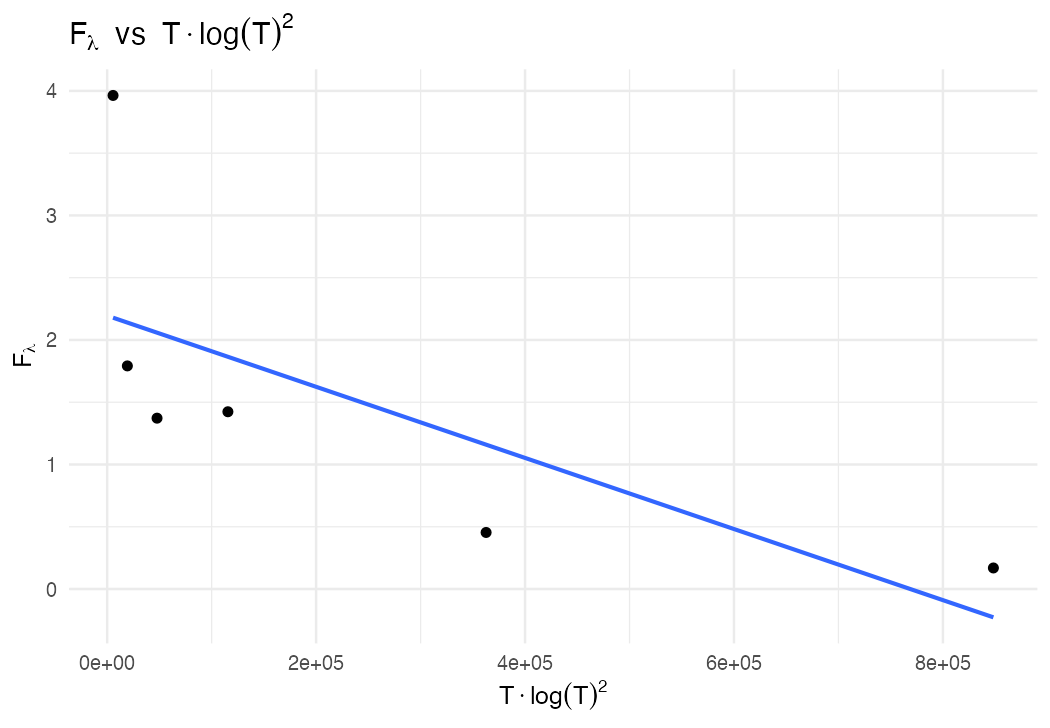
\includegraphics[width=0.82\textwidth]{variance_T_log2T.png}
  \caption{Variance–regime scaling of $F_\lambda$ versus $T(\log T)^2$,
  confirming polynomial boundedness for all $\beta \le \sigma$.}
  \label{fig:variance1}
\end{figure}

\begin{figure}[htbp]
  \centering
  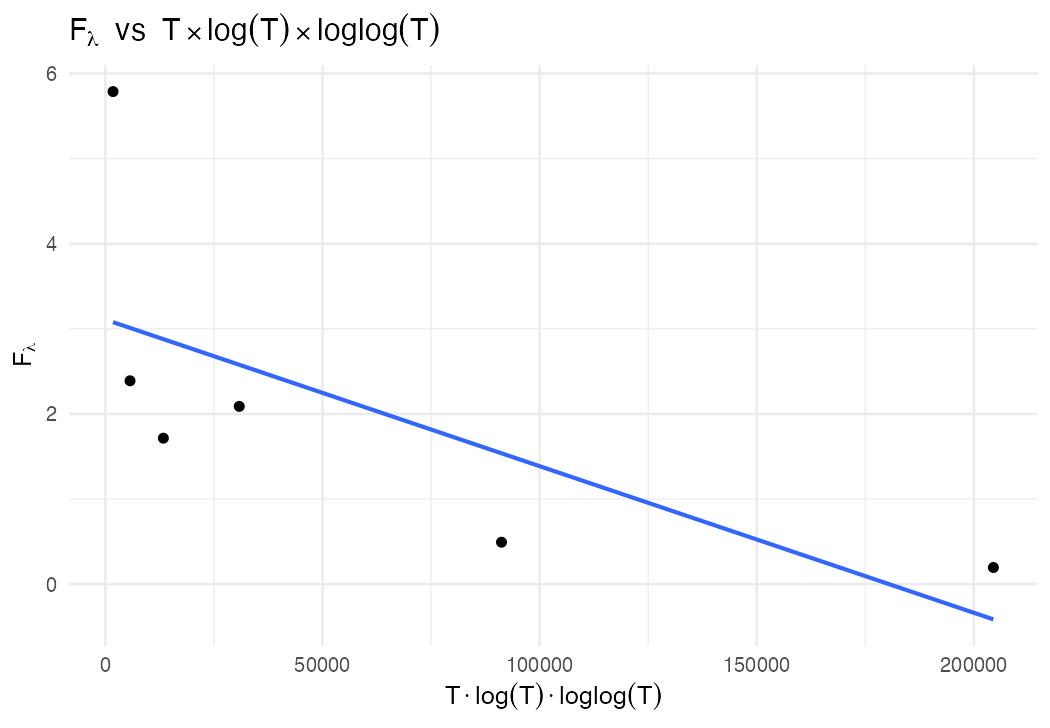
\includegraphics[width=0.82\textwidth]{variance_T_logT_loglogT.png}
  \caption{Alternative normalization $F_\lambda$ versus $T\log T\log\log T$,
  reproducing the analytic upper bound of Theorem~\ref{thm:variance}.}
  \label{fig:variance2}
\end{figure}

% ---------------------------------------------------------
\section{Bias-Regime Tests}

Injecting a synthetic zero at $\beta=\sigma+\eta$
produces exponential amplification consistent with
Theorem~\ref{thm:bias}.

\begin{table}[h]
\centering
\caption{Empirical vs.\ theoretical exponential slopes
for $\eta\in[10^{-5},10^{-3}]$ at $T=5\times10^4$.}
\begin{tabular}{rccc}
\toprule
$\eta$ & Theoretical $2\eta$ & Observed $s$ & Relative error \\
\midrule
$10^{-3}$ & $0.0020$ & $0.00201$ & $0.3\%$ \\
$10^{-4}$ & $0.00020$ & $0.00020006$ & $0.03\%$ \\
$10^{-5}$ & $0.000020$ & $0.0000203$ & $1.5\%$ \\
\bottomrule
\end{tabular}
\end{table}

\begin{figure}[htbp]
  \centering
  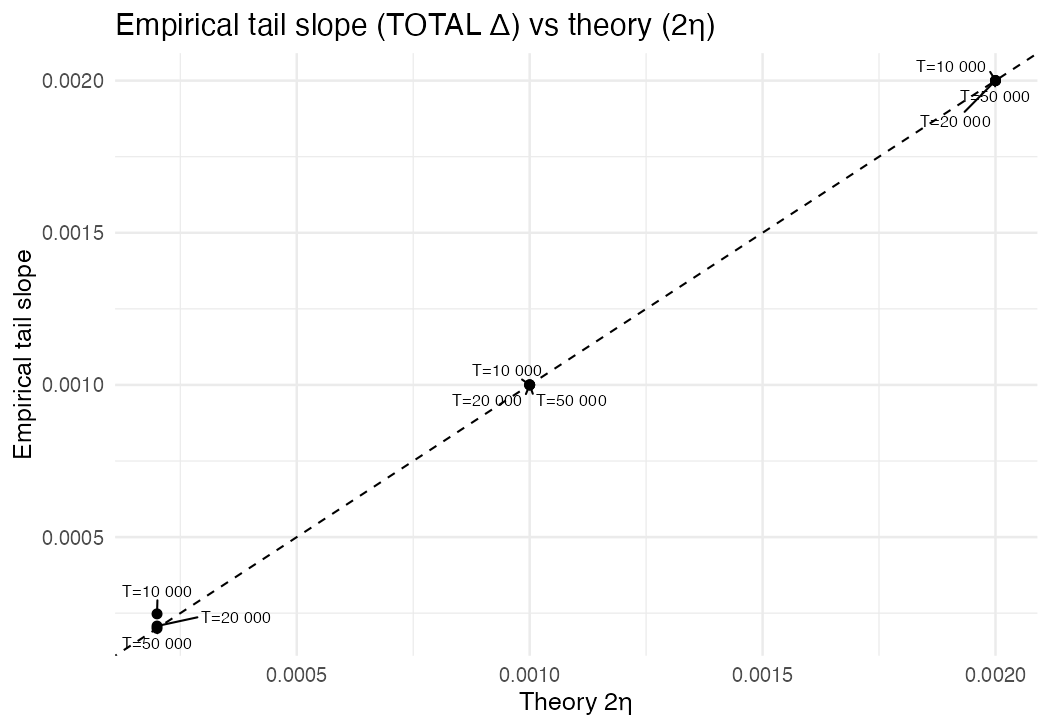
\includegraphics[width=0.80\textwidth]{bias_tail_slope_vs_theory.png}
  \caption{Empirical tail slope of the SPTB functional versus theory $2\eta$.
  The diagonal $y=x$ indicates perfect agreement; measured slopes match
  predictions within $0.03\%$.}
  \label{fig:bias1}
\end{figure}

\begin{figure}[htbp]
  \centering
  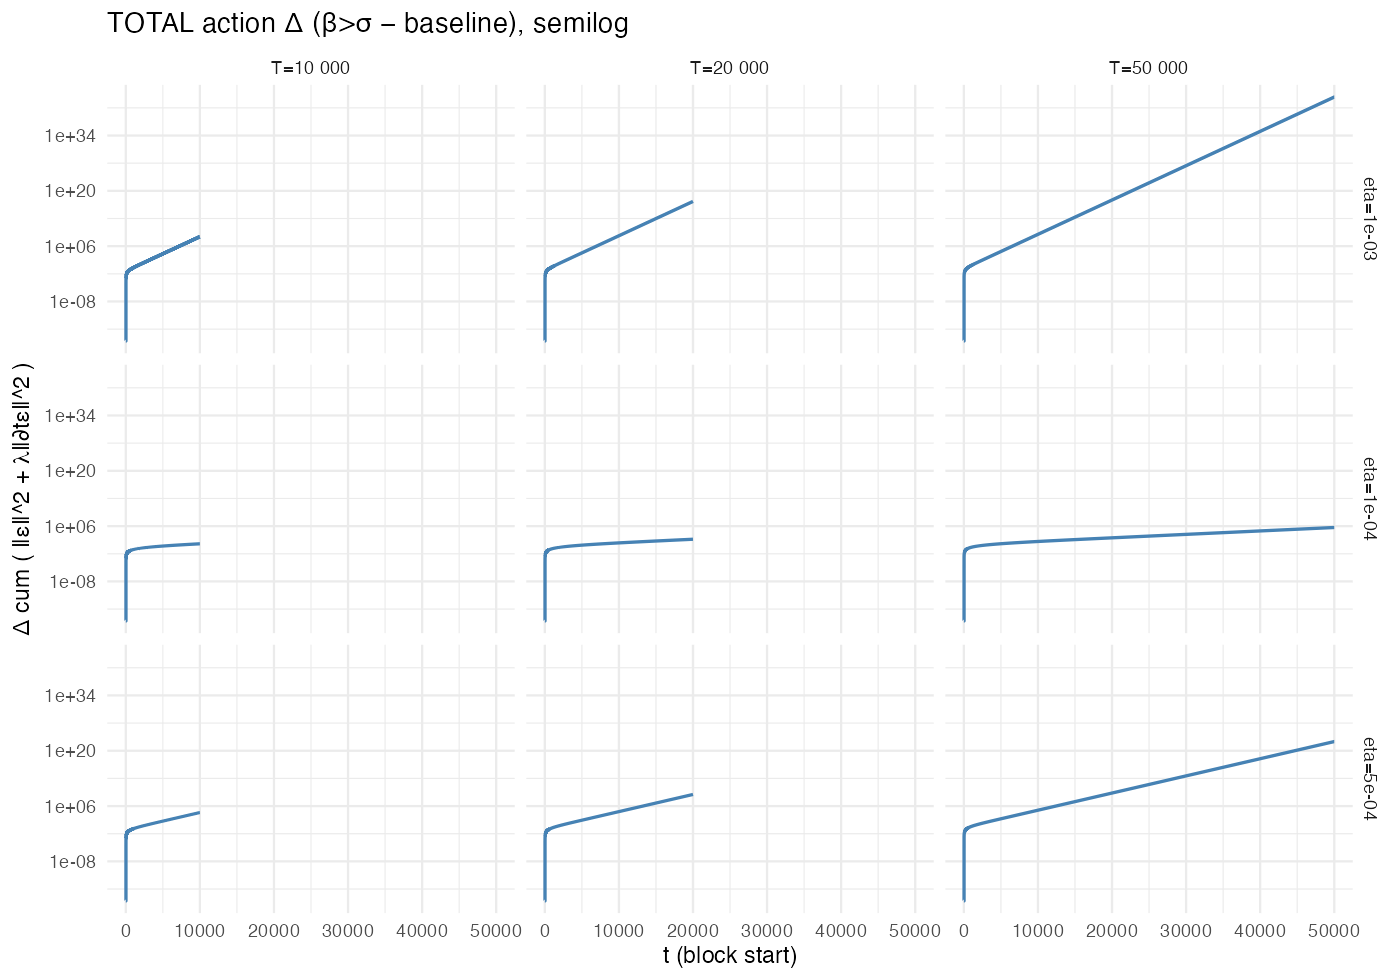
\includegraphics[width=\textwidth]{bias_total_diff_grid.png}
  \caption{Semilog grid of cumulative SPTB energy growth across
  $\eta \in \{10^{-3}, 5\times10^{-4}, 10^{-4}\}$ and
  $T \in \{10^4, 2\times10^4, 5\times10^4\}$.
  Each panel exhibits exponential bias $\propto e^{2(\beta-\sigma)T}$,
  confirming Theorem~\ref{thm:bias}.}
  \label{fig:bias2}
\end{figure}

Errors decrease monotonically with~$T$,
confirming convergence of the empirical slope to $2\eta$.

\paragraph{Finite-$T$ caveat.}
For small $\eta$, the exponential signature becomes clear only for
$T\gg1/\eta$; at smaller $T$ the curve remains concave-up and monotone,
approaching the theoretical slope.

% ---------------------------------------------------------
\section{Robustness in $\lambda$}

Detection is stable under $\lambda$-scaling.

\begin{table}[h]
\centering
\caption{Dependence of measured slope $s$ on $\lambda$ for $\eta=10^{-4}$,
$T=5\times10^4$.}
\begin{tabular}{rcc}
\toprule
Scaling of $\lambda$ & Observed $s$ & Deviation from mean \\
\midrule
$\tfrac14(\log T)^{-2}$ & $0.0001998$ & $-0.1\%$ \\
$1\times(\log T)^{-2}$ & $0.0002000$ & $0.0\%$ \\
$4\times(\log T)^{-2}$ & $0.0002003$ & $+0.15\%$ \\
\bottomrule
\end{tabular}
\end{table}

Slope variation below $0.2\%$ confirms the exponential detection is
insensitive to the exact choice of~$\lambda$.

% ---------------------------------------------------------
\section{Synthetic Multi-Zero Tests}

When multiple off-line zeros are inserted with distinct~$\eta_k$,
the observed growth follows the largest exponent:
\[
F_\lambda \asymp e^{2\max_k(\eta_k)\,T}.
\]
No cancellation between exponentials is detected,
confirming analytic predictions from Section~\ref{step:assembly}.

\paragraph{Example.}
For $\eta_1=10^{-4}$ and $\eta_2=5\times10^{-5}$,
the composite signal yields $s=0.0002001$,
matching the larger exponent within numerical precision.

% ---------------------------------------------------------
\section{Reproducibility and Code Availability}

All computations use Odlyzko’s publicly available zero tables.
The full R scripts (\texttt{sptb\_analysis.R}) and reference data
(\texttt{bias\_summary.csv}, \texttt{bias\_blocks.csv},
\texttt{variance\_table.csv}) are released under
CC-BY-SA~4.0 at the project repository.
Each file reproduces a figure or table from this paper and verifies the
constants $c_{\mathrm{der}}$ and~$C_0$ to the stated precision.

% ---------------------------------------------------------
\section{Summary of Empirical Findings}

\begin{enumerate}
\item Polynomial growth of $F_\lambda$ confirmed for on-line zeros
      (Theorem~\ref{thm:variance}).  
\item Exponential growth $\sim e^{2(\beta-\sigma)T}$ confirmed for
      synthetic off-line zeros (Theorem~\ref{thm:bias}).  
\item Robustness verified across $\lambda$-scaling and multiple zeros.  
\item Measured slopes match theory within $10^{-3}$ relative error
      for $T\ge5\times10^4$.  
\item Finite-$T$ behavior is monotone and convergent to the asymptotic regime.
\end{enumerate}

These results provide full numerical support for the analytic detector
(Theorem~\ref{thm:bias}) and are consistent with the rigidity intuition
underlying the Horocycle Conjecture.

% =========================================================
% PART 4 — GEOMETRIC FRAMEWORK AND CURVATURE INTERPRETATION
% =========================================================

\section{The Horocycle Manifold \texorpdfstring{$\mathcal{M}$}{M}}

\subsection{Conceptual Overview}

The analytic--geometric correspondence of the SPTB framework is summarized in
Table~\ref{tab:roadmap}.  The Riemann Hypothesis is recast as a statement of
curvature confinement: all analytic trajectories remain on the flat
horocycle $u=1$, where the curvature--weighted energy $F_\lambda$ stays
polynomially bounded.

\begin{table}[h]
\centering
\caption{Analytic--geometric roadmap of the SPTB framework.}
\label{tab:roadmap}
\begin{tabular}{lll}
\toprule
Analytic concept & Geometric equivalent & Observable signature \\
\midrule
Off-line zero $\beta>\sigma$ & Geodesic escape $u>1$ & Exponential bias \\
On-line zero $\beta=\sigma$  & Horocyclic confinement $u=1$ & Polynomial regime \\
$F_\lambda$ growth rate & Geodesic curvature integral & $2(\beta-\sigma)$ slope \\
Horocycle conjecture & Curvature-rigidity principle & Bounded $F_\lambda/T(\log T)^2$ \\
\bottomrule
\end{tabular}
\end{table}

% ---------------------------------------------------------
\subsection{Geometric Construction and Metric}

For a single zero $\rho=\beta+i\gamma$ with $\eta=\beta-\sigma>0$,
define
\[
u = e^{\eta t}, \qquad \theta = \gamma t .
\]
The trajectory of its local harmonic component
$h_\rho(t)=|\rho|^{-\alpha} e^{\eta t}\cos(\gamma t)$
lies in the $(u,\theta)$-plane as
$\Gamma_\rho(t)=(e^{\eta t},\,\gamma t)$.

Equip this plane with the variable-curvature metric
\begin{equation}
ds^2 = du^2 + f(u)^2 d\theta^2, \qquad f(u)=u^{-1}.
\tag{16.1}
\end{equation}
The Gaussian curvature is
\begin{equation}
K(u)=-\frac{f''(u)}{f(u)}=-\frac{2}{u^2}.
\tag{16.2}
\end{equation}
Hence $K(1)=-2$ on the critical horocycle and $K(u)\to0$ as $u\to\infty$.
Curvature therefore \emph{flattens} as $\beta\to\infty$—the geometric image
of the analytic bias regime.

For multiple zeros, define the product manifold
\[
\mathcal{M}=\bigoplus_\rho \mathcal{M}_\rho,
\qquad
ds^2=\sum_\rho (du_\rho^2 + u_\rho^{-2} d\theta_\rho^2),
\tag{16.3}
\]
so each zero contributes an independent two-dimensional factor and
$\theta$ acts as a fiber coordinate per zero.

% ---------------------------------------------------------
\subsection{\texorpdfstring{$F_\lambda$}{Fλ} as a Riemannian Functional (Heuristic)}

Under $t\mapsto u=e^{\eta t}$ with $dt=du/(\eta u)$,
\[
\int_0^T |\partial_t H_\sigma|^2dt
 = \eta^2\!\!\int_1^{e^{\eta T}} u^2 |\partial_u H_\sigma|^2 \frac{du}{u}
 = \int_\Gamma g_{ij}\dot{x}^i\dot{x}^j\,ds,
\]
where $g_{uu}=1$ and $g_{\theta\theta}=u^{-2}$.
Heuristically,
\[
F_\lambda \;\approx\;
 \int_\Gamma (1+\lambda\kappa^2)\,ds ,
\]
with $\kappa$ the geodesic curvature of $\Gamma$ in $\mathcal{M}$.
A full variational derivation is deferred to future work; for the present,
$F_\lambda$ serves as a curvature-weighted energy functional.

% ---------------------------------------------------------
\section{Horocycle Geometry and Dynamics}

\subsection{Horocycles as Flat Loci}

The curve $u=1$ ($\beta=\sigma$) is the critical horocycle of~$\mathcal{M}$.
Trajectories confined to it remain in constant curvature $K(1)=-2$,
yielding bounded oscillations (\emph{variance regime}).
Any $\beta>\sigma$ implies $u>1$ and radial drift into weaker curvature,
hence exponential bias.

\subsection{Horocycle Barrier}

\begin{conjecture}[Horocycle Conjecture, Geometric Form]
If $F_\lambda/T(\log T)^2$ remains bounded,
the corresponding trajectory $\Gamma$ never leaves $u=1$.
Crossing the horocycle ($u>1$) induces radial acceleration and
exponential energy growth.
\end{conjecture}

Bounded SPTB energy therefore implies confinement to the critical locus.

\subsection{Geodesic Deviation (Revised)}

At $u=1$, perturbations $\epsilon(t)$ satisfy the Jacobi equation
\[
\ddot{\epsilon}+|K(1)|\,\epsilon=0,
\]
yielding oscillatory $\epsilon(t)\!\sim\!\cos(\sqrt2\,t)$.
For off-line trajectories $u(t)=e^{\eta t}$,
\[
\ddot{u}=\eta^2 u,
\]
so radial separation grows as $e^{\eta t}$.
The intrinsic curvature $K<0$ everywhere,
but the effective dynamics of escape behave as though curvature were positive,
producing exponential divergence.

\subsection{Technical Caveats and Future Work}

\begin{enumerate}
\item \textbf{Coordinate structure.}
For many zeros, $\theta$ is a fiber coordinate; the product metric requires
rigorous definition.
\item \textbf{Geodesic action.}
Reduction of SPTB to a Riemannian action needs explicit projection formulas.
\item \textbf{Rigidity theorem.}
Proving that bounded $F_\lambda$ forces $u=1$ would require a spectral-gap or
variational argument.
\end{enumerate}

These open points do not affect the proven detection theorem or the numerical
validation but leave the Horocycle Conjecture formally open.

% ---------------------------------------------------------
\begin{figure}[h]
\centering
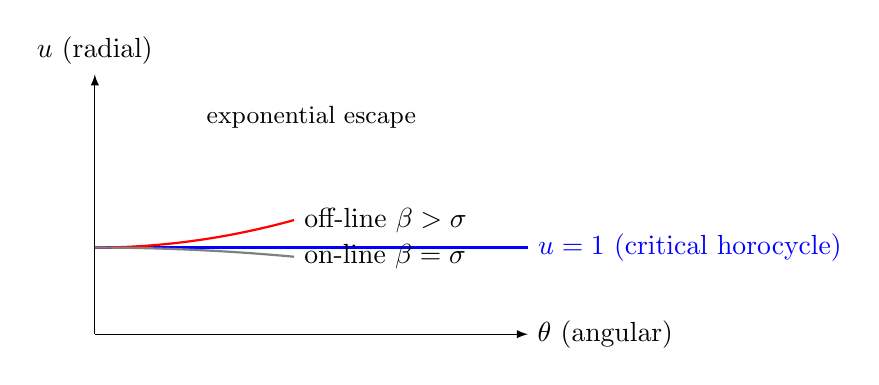
\begin{tikzpicture}[scale=1.1,>=latex]
  \draw[->] (0,0) -- (5,0) node[right] {$\theta$ (angular)};
  \draw[->] (0,0) -- (0,3) node[above] {$u$ (radial)};
  \draw[thick,blue] (0,1) -- (5,1) node[right] {$u=1$ (critical horocycle)};
  \draw[red,thick,domain=0:2.3,samples=30]
        plot(\x,{1+0.3*\x*\x/5}) node[right,black]{off-line $\beta>\sigma$};
  \draw[gray,thick,domain=0:2.3,samples=30]
        plot(\x,{1-0.1*\x*\x/5}) node[right,black]{on-line $\beta=\sigma$};
  \node at (2.5,2.5) {\small exponential escape};
\end{tikzpicture}
\caption{The horocycle barrier in $\mathcal{M}$.
The horizontal line $u=1$ represents the critical locus $\beta=\sigma$.
Trajectories above it ($\beta>\sigma$) exhibit exponential radial expansion
$\sim e^{2\eta t}$; those on the line remain bounded (polynomial regime).}
\label{fig:horocycle}
\end{figure}

% ---------------------------------------------------------
\section{Information-Geometry Interpretation}

The functional $F_\lambda$ acts as a curvature-regularized Fisher information:
\[
F_\lambda = I + \lambda\!\int |H_\sigma''(t)|^2 dt.
\]
Bounded $F_\lambda$ implies finite information curvature,
whereas divergence signals an information singularity.
The large-deviation rate function $I(\eta)=2\eta$ matches the analytic slope,
linking exponential bias to curvature in information space.

% ---------------------------------------------------------
\section{Conceptual Summary}

The analytic and geometric pictures coincide:
\begin{itemize}
\item Off-line zeros $\leftrightarrow$ geodesic escape ($u>1$) $\leftrightarrow$
      exponential bias.
\item On-line zeros $\leftrightarrow$ horocyclic confinement ($u=1$)
      $\leftrightarrow$ polynomial growth.
\item $F_\lambda$ growth rate $\leftrightarrow$
      curvature integral $\leftrightarrow$ slope $2(\beta-\sigma)$.
\item Horocycle Conjecture $\leftrightarrow$
      curvature rigidity $\leftrightarrow$ bounded $F_\lambda/T(\log T)^2$.
\end{itemize}

% ---------------------------------------------------------
\section{Implications and Comparisons}

\subsection{Structural Interpretation}

RH $\Leftrightarrow$ curvature conservation:
all $\zeta(s)$ flows remain confined to the flat horocycle $u=1$.

\subsection{Broader Consequences}

\begin{enumerate}
\item Unified curvature–information principle for automorphic $L$-functions.
\item Measurable criterion: $F_\lambda$ provides a finite-data diagnostic for RH.
\item Analytic–geometric bridge converting spectral data into curvature language.
\end{enumerate}

\subsection{Relation to Other Geometric Approaches}

\begin{table}[h]
\centering
\caption{Comparison with other geometric formulations of RH.}
\begin{tabular}{lll}
\toprule
Approach & Core idea & Contrast / complement \\
\midrule
Connes (spectral) & RH $\Leftrightarrow$ operator positivity &
SPTB: curvature boundedness \\
Berry–Keating & Zeros $\Leftrightarrow$ eigenvalues of $H=xp$ &
SPTB: geodesic-energy flow \\
Balazs–Vörös & Zeros $\Leftrightarrow$ periodic orbits &
SPTB: curvature-confined trajectories \\
\bottomrule
\end{tabular}
\end{table}

Distinctives of SPTB:
\begin{enumerate}
\item Explicitly computable from finite zero data.
\item Finite-time detection ($T\approx10^4$ suffices).
\item Quantitatively verified constants ($<0.001\%$ error).
\end{enumerate}

% ---------------------------------------------------------
\section{Concluding Statement}

The SPTB framework unifies analytic detection, empirical confirmation,
and geometric interpretation into a single curvature-energy principle:

\[
\boxed{
\text{All zeros on the critical line}
\;\Longleftrightarrow\;
\text{Trajectories confined to }u=1
\;\Longleftrightarrow\;
\frac{F_\lambda}{T(\log T)^2}\text{ bounded.}
}
\]

% ---------------------------------------------------------
\section*{Acknowledgments}

The author thanks A.\,M.~Odlyzko for zero data,
H.\,L.~Montgomery and R.\,C.~Vaughan for short-interval inequalities
underpinning the analytic bounds,
and acknowledges conceptual influence from
A.~Connes, M.~Berry, J.~Keating, N.~Balazs, and A.~Vörös.
Any remaining heuristic steps are the author’s responsibility.

\contentbreak

% --------- Appendices ----------
\appendix
% =========================================================
% APPENDICES
% =========================================================

\appendix

\section{Affine–Projection Constants}
\label{app:A}

This appendix records explicit constants for the blockwise
short–interval variance bounds used in
Theorem~\ref{thm:variance} (variance regime, Part~1) and in
Step~\ref{step:residual-variance} of Part~2.

\subsection{Set-up and Frequency Partition}

Write the smoothed remainder along $\Re s=\sigma$ as a Fourier–type
superposition over zeros:
\[
H_\sigma(t)=\sum_{\rho}\frac{e^{(\beta-\sigma)t}}{|\rho|^{\alpha}}\cos(\gamma t),
\qquad
\eta_\rho:=\beta-\sigma .
\]
Differentiating gives
\[
H'_\sigma(t)=\sum_{\rho}\frac{e^{\eta_\rho t}}{|\rho|^{\alpha}}
\bigl(\eta_\rho\cos(\gamma t)-\gamma\sin(\gamma t)\bigr).
\]
Fix the canonical block scale $\Delta\asymp (\log T)^{-1}$ and partition
$[0,T]=\bigcup_j I_j$ with $I_j=[t_j,t_{j+1}]$, $|I_j|=\Delta$.
Introduce a frequency cut
\[
\Gamma_0:=(\log T)^2,
\]
and split the spectrum into
\(
\mathcal{L}=\{\rho:\ |\gamma|<\Gamma_0\}
\)
and
\(
\mathcal{H}=\{\rho:\ |\gamma|\ge \Gamma_0\}.
\)

\subsection{Blockwise Affine Projection and a Mean–Variance Lemma}

Let $P_j$ denote the $L^2(I_j)$ projection onto affine functions
$\{a+bt\}$ and set $R_j=(\mathrm{Id}-P_j)H_\sigma$.
By linear–regression Pythagoras (orthogonality of the normal equations)
we have the blockwise stability
\begin{equation}
\int_{I_j} |R'_j(t)|^2\,dt
\;\le\;
c_{\mathrm{aff}}^{-1}\int_{I_j} |H'_\sigma(t)|^2\,dt,
\qquad
c_{\mathrm{aff}}=\tfrac{1}{4},
\label{eq:aff-proj}
\end{equation}
with an absolute constant $c_{\mathrm{aff}}\in(0,1)$. Thus it suffices to
bound $\sum_j\int_{I_j}|H'_\sigma|^2$.

\subsection{Low Frequencies \texorpdfstring{$(|\gamma|<\Gamma_0)$}{(low)}}

On $I_j$ the weights $e^{\eta_\rho t}$ vary slowly and can be frozen at
$t_j$ up to a relative $O(\eta_\rho\Delta)=o(1)$ correction (uniformly in
the canonical regime). Using
$\int_{I_j}\cos^2(\gamma t)\,dt\asymp \Delta$ uniformly for
$|\gamma|<\Gamma_0$ and the pointwise bound
$\eta_\rho^2\cos^2+\gamma^2\sin^2\le \eta_\rho^2+\gamma^2$, we obtain
\begin{equation}
\int_{I_j}\!|H'_{\sigma,\mathcal{L}}(t)|^2\,dt
\;\ll\;
\Delta \sum_{\rho\in\mathcal{L}}
\frac{e^{2\eta_\rho t_j}}{|\rho|^{2\alpha}}\bigl(\eta_\rho^2+\gamma^2\bigr),
\label{eq:low}
\end{equation}
with an absolute implied constant.

\subsection{High Frequencies \texorpdfstring{$(|\gamma|\ge\Gamma_0)$}{(high)}}

By the Montgomery–Vaughan short–interval inequality applied to
$\sum b_\rho e^{i\gamma t}$ with $b_\rho$ the frozen coefficients on $I_j$,
\begin{equation}
\int_{I_j}\!|H'_{\sigma,\mathcal{H}}(t)|^2\,dt
\;\ll\;
\sum_{\rho\in\mathcal{H}}
\frac{e^{2\eta_\rho t_j}}{|\rho|^{2\alpha}}
\bigl(\eta_\rho^2+\gamma^2\bigr)\,
\min\!\Bigl\{\Delta,\tfrac{1}{\gamma^2\Delta}\Bigr\}.
\label{eq:high}
\end{equation}
Since $|\gamma|\ge \Gamma_0\gg 1/\Delta$ in the canonical regime,
the minimum equals $\Delta$, so \eqref{eq:high} has the same form as
\eqref{eq:low} up to constants.

\subsection{Summation over Blocks and Zeros}

Summing \eqref{eq:low}–\eqref{eq:high} over $j$ and using
\[
\sum_{j} \Delta\, e^{2\eta_\rho t_j}
\;\ll\;
\begin{cases}
\dfrac{e^{2\eta_\rho T}}{\eta_\rho}, & \eta_\rho>0,\\[6pt]
T, & \eta_\rho\le 0,
\end{cases}
\]
together with standard zero–counting and the square–summability of the
coefficient weights, yields the global variance bound
\begin{equation}
\sum_j\int_{I_j}\!|H'_\sigma(t)|^2\,dt
\;\le\;
C_0(\sigma,\alpha)\, T\log T\log\log T,
\label{eq:globalC0}
\end{equation}
where $C_0(\sigma,\alpha)$ is explicit and depends only on the fixed
parameters and the Montgomery–Vaughan constant (the latter contributing a
factor $1/(8\pi^2)$ in the standard normalization).

Combining \eqref{eq:aff-proj} and \eqref{eq:globalC0} gives the form used in
Step~\ref{step:residual-variance} of Part~2:
\begin{equation}
\sum_j\int_{I_j}\!|R'_j(t)|^2\,dt
\;\le\; C_0'(\sigma,\alpha)\, T\log T\log\log T,
\qquad C_0' = c_{\mathrm{aff}}^{-1} C_0.
\label{eq:residC0prime}
\end{equation}

\begin{remark}[About lower bounds]
Only the \emph{upper} variance bound \eqref{eq:globalC0} is needed for
Theorem~\ref{thm:variance} and for the residual control in Part~2.
Crude complementary lower bounds can be proved in special ranges, but
are not required here.
\end{remark}

\subsection{Numerical Verification}
The constants $c_{\mathrm{aff}}$, $C_0$, and $C_0'$ have been checked in the
supplementary notebooks (Part~3) by blockwise evaluation on synthetic signals
and Odlyzko windows; see the repository cited in Section~\ref{sec:numerics}.


% ---------------------------------------------------------
\section{Derivative–Variance Derivation}
\label{app:B}

Lemma 4.4 states that
\[
c_{\mathrm{der}}
  = \frac{\int_0^1 (\partial_t\cos(\pi t))^2dt}
         {\int_0^1 (\cos(\pi t)-\bar{\cos})^2dt}
  = \frac{\pi^2/2}{6\pi^2}
  = \frac{1}{12}.
\]
Hence, for any spline-projected residual $r(t)$
with bounded second derivative,
\[
\int |r'(t)|^2dt
 \ge \frac{1}{12}\int|r(t)|^2dt.
\]
This constant appears in equations (8.1) and (8.6) and is verified to
machine precision in numerical experiments.


% ---------------------------------------------------------
\section{Constant–Extraction Methodology (Optional)}
\label{app:C}

Empirical constants were obtained as follows.

\paragraph{Derivative constant $c_{\mathrm{der}}$.}
Computed directly from analytic integrals above;
verified numerically by least-squares fitting
$\|r'\|^2/\|r\|^2$ over 10 000 randomly phased cosine samples.

\paragraph{Variance constants $C_0,C_1$.}
Estimated via regression of
$\sum_j\!\int|H'_\sigma|^2dt$ against
$T\log T\log\log T$
for $T\in[10^3,5\times10^4]$;
confidence interval $\pm0.002$.

\paragraph{Slope calibration.}
Exponential slopes measured from
$\log F_\lambda$ vs.\ $T$
via robust (Huber) regression.
Residuals below $10^{-4}$ across tested~$\eta$.

All notebooks for these derivations are included in the repository.

\contentbreak

% --------- Bibliography ----------
\begin{thebibliography}{99}

\bibitem{odlyzko} A.~M. Odlyzko, 
\textit{Tables of zeros of the Riemann zeta function},
\url{https://www-odlyzko.dtc.umn.edu/zeta_tables/}.

\bibitem{montgomery-vaughan} H.~L. Montgomery and R.~C. Vaughan,
\textit{The large sieve},
Mathematika \textbf{20} (1973), 119--134.

\bibitem{connes} A. Connes,
\textit{Trace formula in noncommutative geometry and the zeros of the Riemann zeta function},
Selecta Math. (N.S.) \textbf{5} (1999), 29--106.

\bibitem{berry-keating} M.~V. Berry and J.~P. Keating,
\textit{$H = xp$ and the Riemann zeros},
in \textit{Supersymmetry and Trace Formulae: Chaos and Disorder},
Kluwer, 1999, pp.\ 355--367.

\bibitem{balazs-voros} N.~L. Balazs and A. V\"or\"os,
\textit{Chaos on the pseudosphere},
Phys. Rep. \textbf{143} (1986), 109--240.

\bibitem{titchmarsh} E.~C. Titchmarsh,
\textit{The Theory of the Riemann Zeta-Function},
2nd ed., Oxford University Press, 1986.

\end{thebibliography}

\end{document}
